\documentclass[11pt]{article}

\usepackage{url}
\usepackage{hyperref}
\usepackage{graphicx}
\usepackage{verbatim}
\usepackage{color}
\usepackage{upquote}
\usepackage{float}
\usepackage{amsmath}
\usepackage{mwe}
\usepackage{subcaption}

\setlength{\parskip}{0.5cm plus4mm minus3mm}
\captionsetup{font=footnotesize}


\textwidth=6.4in
\textheight=8.5in
\hoffset=-0.7in
\voffset=-0.7in

\setlength{\parindent}{0cm} 

\newcommand{\Yfun}{Y}
%\newcommand{\TAG}{test}
\newcommand{\TAG}{\begin{color}{blue}This tutorial is currently under construction. Please check back later for more by keeping your software updated.\end{color}}

\newcommand{\HERE}{\begin{color}{blue}Currently working on this part.\end{color}}

\hyphenation{Text-Wrangler}

\title{Chapter 2: Introduction to Slepian Functions}
\author{Sarah Kroeker, Alain Plattner}

\begin{document}
\maketitle

After having worked through Chapter 1: Introduction to Spherical
Harmonics, we will now have a look at what spherical Slepian functions
are. The goal of this chapter is not to give a solid foundation of the
mathematical intricacies. This can be obtained from the many research
articles in the literature. Rather, we will look at some basic ideas
and plot the first few Slepian functions.


\section{Basic ideas}
When plotting spherical harmonics in chapter 1, it became clear that
all of these spherical harmonics are functions that cover the entire
sphere. This is of course an advantage if we try to describe functions
(or maps), that cover the entire planet, such as gravity fields,
magnetic fields, etc. We saw in chapter 1 that we can generate pretty
much any spatial pattern we like by simply summing up different
spherical harmonics each multiplied by a different factor called
``coefficient''.

But what can we do if we only have information within a specific
region? Sometimes it's fine to just describe that information as
point values. But in some cases, as for example when we measure
gravity or magnetic data at satellite altitude, and we want to
calculate, what the corresponding magnetic or gravity field looks like
on the planet's surface (assuming there are no gravity or magnetic
sources between the planet and the satellite, or that they are
negligible), we need to describe these fields in spherical harmonics.

This is where the Slepian functions come in. Slepian functions are
linear combinations of spherical harmonics which means that they are
constructed by multiplying each spherical harmonic function with a
factor (called Slepian coefficient) and then adding them all up. The name
Slepian function stems from the first author of a research article,
that described the original idea for 1-dimensional functions.

There are different types of Slepian functions that are constructed in
different ways but the basic idea is always to solve an optimization
problem, in which we try to balance the number of spherical-harmonic
functions we use (the maximum spherical-harmonic degree) in the
construction of the Slepian functions, and how much they are
concentrated within the region that we are interested in.

\section{Classical Scalar Slepian Functions}
%A brief mathematical overview will be as follows; for a more in depth treatment, please see Section 2.3 of Simons and Plattner (2014): \\
%\url{https://pdfs.semanticscholar.org/886c/70532a885ca66c1b70e55eb65a3f6500be67.pdf}.
%
Let's first look at the classical scalar Slepian functions, which are spectrally limited and spatially optimized. These functions are suitable to use when you are limited to information within a specific region as mentioned above, but only when that information is constrained to the surface of the sphere as point values; classical vector Slepian functions will be addressed in a later chapter after a discussion of vector spherical harmonics. The Slepian functions are bandlimited by the maximum spherical harmonic degree \textit{L} for region of concentration \textit{R}. We will choose our region to be the continent \textbf{Africa} for our first example. The following examples will include a region of an axisymmetric polar cap, a polar ring, and a polar cap when rotated away from the north pole.

\subsection{Calculating Coefficients for a Region}

In the Slepian folder start MATLAB and run: 

\verb|demos_chapter_two(2.1)|

You may also find it helpful to open \verb|demos_chapter_two.m| in a text editor and browse the script as you read through this tutorial. The demo file is divded into cases for each subsection of this chapter. 

The function \verb+glmalpha+ is used to calculate unit-normalized spherical harmonic coefficients given the following required inputs:

\verb+		TH+ - a desired region (in this example: \verb+'africa'+)

\verb+		L+ - the bandwidth, or maximum spherical harmonic degree. 

If you find the program running too slowly for the purpose of quickly going through this tutorial or freezing up in MATLAB you may need to edit the demo file and set \verb|L| in \verb|glmalpha()| to a smaller value, say 5 for example.

Thus the output of \verb+glmalpha+ we used for this example is:

\verb+		G+ - a unitary matrix of localization coefficients. 

There are several other inputs and outputs that may and should be used later; see \verb+help glmalpha+ for more details. 

We specify one other input to indicate the ordering of the spherical harmonic coefficients. In our codes  we use two different methods of ordering: ADDMOUT and ADDMON. 

Remember that spherical harmonics have a degree $l$ and an order $m$. Degrees are all integers greater than zero and orders for each degree vary between $-l$ and $l$.

We could order these spherical harmonics as


\begin{tabular}{c|cccccccccc}
l&0&1&1&1&2&2&2&2&2&etc.\\
\hline
m&0&-1&0&1&-2&-1&0&1&2&\text{etc.}
\end{tabular}

This is called the ADDMOUT ordering and is the ordering in which the columns of the Slepian matrices in \verb+glmalpha+, \verb+gradvecglmalpha+, and all these other similar functions are returned.

The other ordering that we may use is:

\begin{tabular}{c|cccccccccc}
l&0&1&1&1&2&2&2&2&2&\text{etc.}\\
\hline
m&0&0&-1&1&0&-1&1&-2&2&\text{etc.}
\end{tabular}

This one we call ADDMON and it is the ordering in which the coefficients from functions like \verb+LocalInnerField+ (which will be discussed in a later chapter) are returned. Every function that returns coefficients or matrices of coefficients should state in their help menu in which format the coefficients are. Just run \verb|help [function]| in MATLAB.

Returning to our example, if you run \verb+help glmalpha+ you will read that it uses the ADDMOUT ordering and thus requires us to use \verb+0+ as the fourth input. We will choose a value of \verb+L=20+. Now we can run:


\verb|		[G] = glmalpha('africa',20,[],0);|

and observe the output \verb+G+ which should be a $(L+1)^2\times(L+1)^2$ orthonormal matrix of coefficients. Each column of \verb+G+ contains a set of coefficients for a single slepian function which are in the ADDMOUT ordering:

$$
G = \begin{bmatrix} 
g_{00,1}  & g_{00,2}  & \dots  & g_{00,(L+1)^2}   \\
g_{1-1,1} & g_{1-1,2} & \dots  & g_{1-1,(L+1)^2}  \\
\vdots    & \vdots    &        & \vdots           \\ 
g_{LL,1}  & g_{LL,2}  & \dots  & g_{LL,(L+1)2}    \\  
\end{bmatrix}
$$

where the subscript of each element contains the $lm$ values and the slepian function number separated by a comma respectively. The first column \verb+G(:,1)+ is the coefficients corresponding to the ``best'' Slepian funtion, or the one that is most spatially concentrated within our chosen region of Africa. \verb+G(:,2)+ would be the second best, \verb+G(:,3)+ would be the third best, and so on until \verb|G(:,(L+1)^2)|.
 
Once the coefficients have been calculated we desire a neutral type of sorting in the format called LMCOSI to prepare for plotting.

In the lmcosi format, we explicitly write out the degrees, orders, and coefficients which in the following I will call $c_{l\,m}$

\begin{tabular}{c c c c}
l&m&co&si\\
\hline
0&0&$c_{0\,0}$&0\\
1&0&$c_{1\,0}$&0\\
1&1&$c_{1\,-1}$&$c_{1\,1}$\\
2&0&$c_{2\,0}$&0\\
2&1&$c_{2\,-1}$&$c_{2\,1}$\\
2&2&$c_{2\,-2}$&$c_{2\,2}$\\
\vdots&\vdots&\vdots&\vdots
\end{tabular}

As you can see this last ordering is an entire matrix instead of just a vector. This is a disadvantage to run calculations but it is less ambiguous than just a vector of coefficients.

Luckily we have programs that take care of these issues. These programs have the creative names
\verb+coef2lmcosi+ and \verb+lmcosi2coef+. You can probably guess from the name what each does.

For our Africa example we will need to feed our coefficients into \verb+coef2lmcosi+ and again tell it whether they are in the ADDMOUT or ADDMON format. This is indicated by using the value 1 for the second input (see \verb+help coef2lmcosi+). The output is saved as \textit{lmcs} but you can name it whatever you would like. Run:

\verb+		lmcs=coef2lmcosi(G(:,1),1);+

The first column of G, or the first Slepian function, is used in our example for simplicity's sake; we show in Section 3 how to make a linear combination of Slepian functions.

We now have one more step before we are ready to plot and that is to evaluate the coefficients using the function \verb+plm2xyz+. The required inputs are our \textit{lmcosi} format matrix and a chosen resolution. You can choose \textit{res}=1, or 0.5, or even 0.1 for a very high resolution image, but keep in mind this will also use much calculation time and memory.  We will give the output the arbitrary name `data' and choose  a resolution of 0.5. Run:

\verb+		data=plm2xyz(lmcs,0.5);+

And finally to plot we will use \verb+plotplm+:

\verb+		plotplm(data,[],[],1,0.5);+

where the fourth input chooses the plotting method. The value '1' corresponds to a Mollweide projection of Earth.

We use \verb+kelicol(1)+ for a more clear color scheme where white sections are of value 0. It is recommended to change the maximum and minimum of the color scheme which you can do by running:

\verb+		caxis([-1,1]*max(abs(caxis)));+

As expected, the fluctuations are concentrated on the center of Africa and negligible elsewhere. The plot produced by \verb|demos_chapter_two(2.1)| should match Figure 1.

\begin{figure}[H]
  \centering
  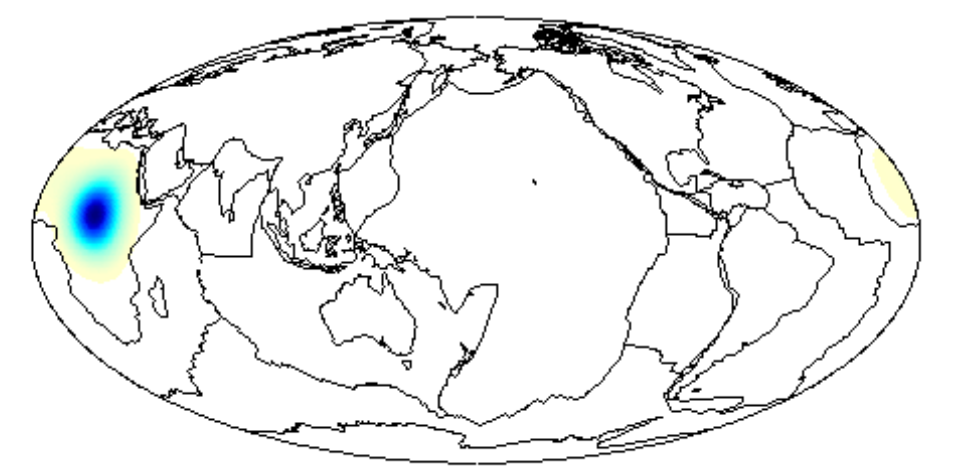
\includegraphics[width=0.5\textwidth]{figures/figure1.png}
  \caption{Result of example using glmalpha() with L=20 to calculate coefficients, plm2xyz() to evaluate them, and plotplm() to plot with method 1 - the Mollweide projection. Only the first ``best" concentrated Slepian function is plotted. The color scheme is kelicol(1) and max/min values are changed to fit the max/min of data plotted.}
\label{figure1}
\end{figure}

\textbf{Anarctica: A Special Case}

[antarctica demo coming soon]

\textbf{Exercise:} Pick a different a region, or subtract a region from Africa to use as the domain and plot again. You can edit \verb|demos_chapter_two.m|, write your own \verb|.m| file, or run line by line in matlab.
 
% clarify that plotplm can take either lmcosi or r lon lat data?

\subsection{Calculating Coefficients for an Axisymmetric Polar Cap}

We now look at the case of an axisymmetric polar cap.

You can run:

\verb|		demos_chapter_two(2.2)|

which will plot both a Mollweide projection, as well as the perspective of looking down at the North Pole.

The functions used for this type of region follow the same format as in section 2.1, however we have changed the inputs of \verb|glmalpha()|. \verb|TH| is now an opening angle in degrees, which we have chosen to be 40, and a value of 1 is passed as the third input to indicate we are creating coefficients for a polar cap of radius \verb|TH|.

To plot as a sphere, a value of 2 for the plotting method should be given to \verb|plotplm()| and then running \verb|view(2)| will rotate the sphere so that the North Pole is pointing out at the viewer.

The demo should produce the same images as Figure 2 below.

\begin{figure}[H]
  \centering
  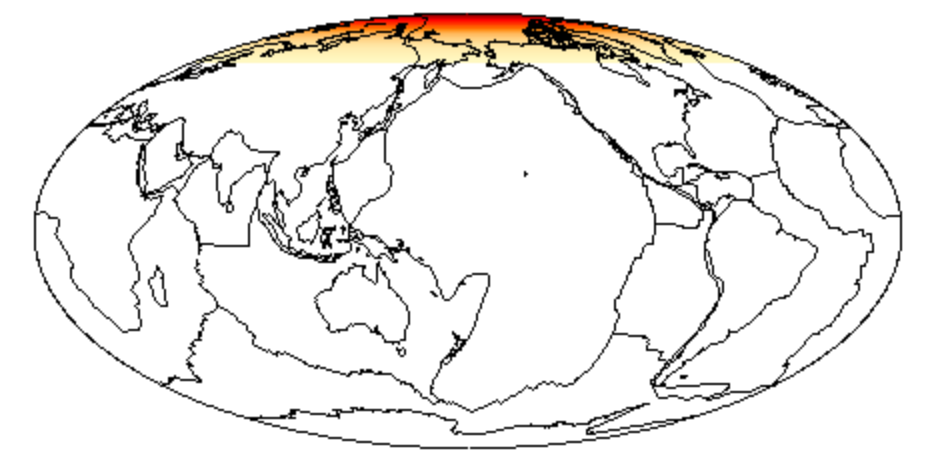
\includegraphics[height=1.2in]{figures/figure2A.png}
  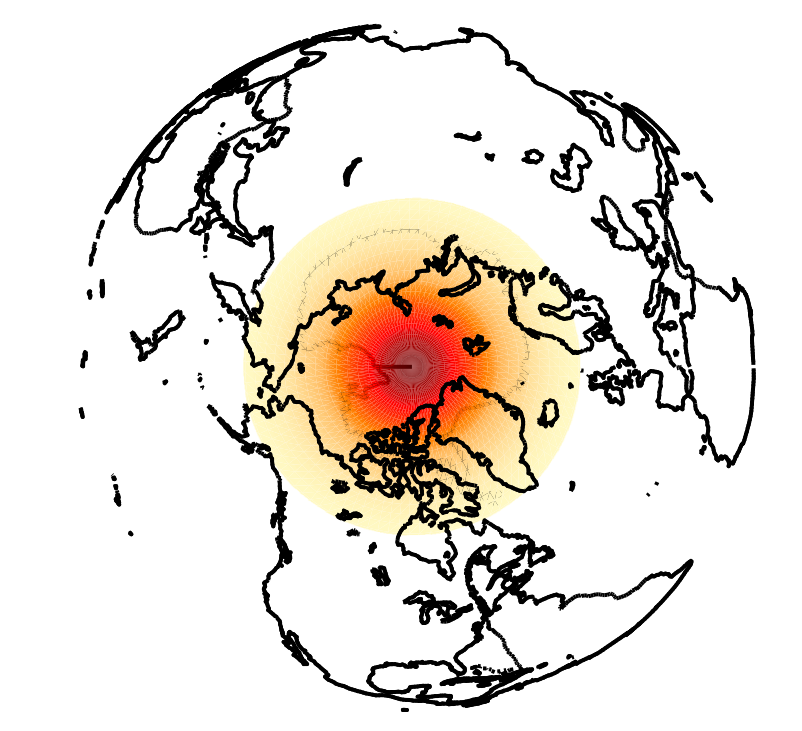
\includegraphics[height=1.2in]{figures/figure2B.png}
  \caption{The first Slepian function of a polar cap of opening angle 40 degrees plotted in both the Mollweide projection (top) and on a sphere with the North pole rotated to the center of the image (bottom).}
   \label{figure2}
\end{figure}

\textbf{Exercise:} The first Slepian function appears roughly symmetric. Try plotting other Slepian functions and see how the distribution changes when they are less concentrated in the specified polar cap.

\subsection{Calculating Coefficients for an Axisymmetric Double Polar Cap}

The double polar cap is very similar to our previous example. The only difference is choosing our third input into \verb|glmalpha()| to be the value 2 to indicate a double polar cap. The opening angle is still chosen to be 40. 

Run:

\verb|		demos_chapter_two(2.3)|

We plot with a Mollweide projection and on the sphere with the view of the North Pole and South pole. 

\begin{figure}[H]
  \centering
  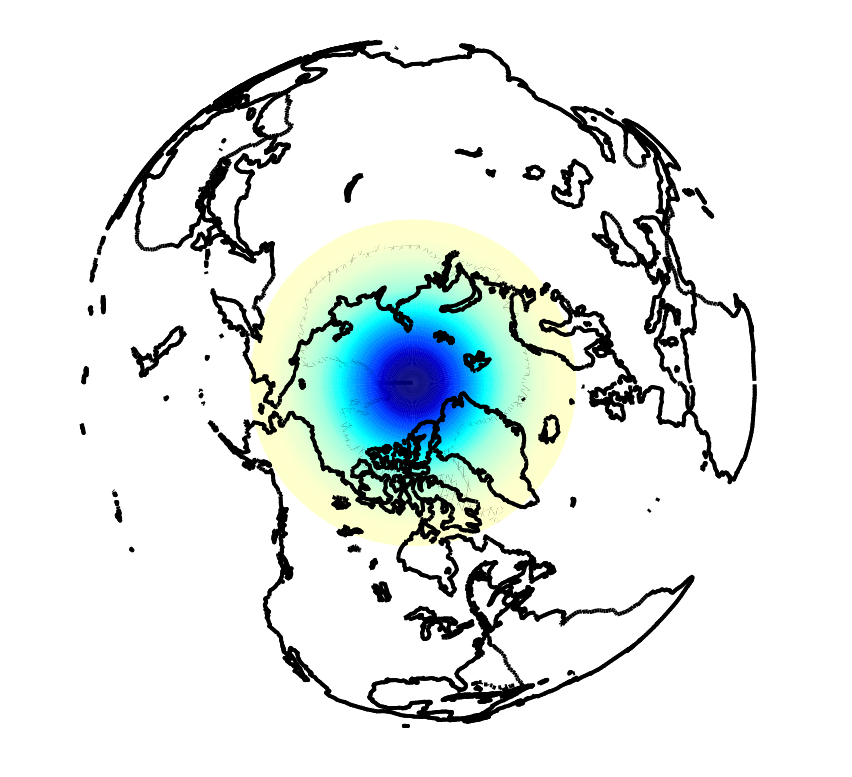
\includegraphics[height=1.2in]{figures/figure3B.png}
  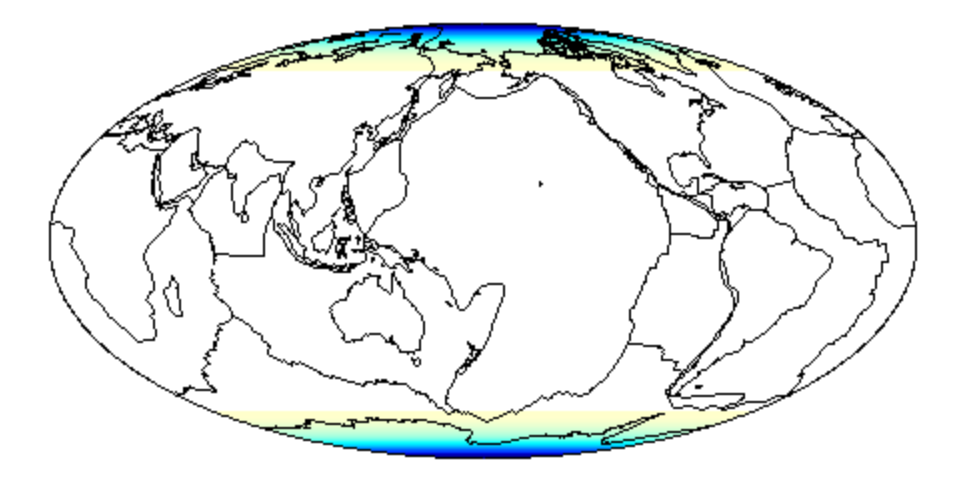
\includegraphics[height=1.2in]{figures/figure3A.png}
  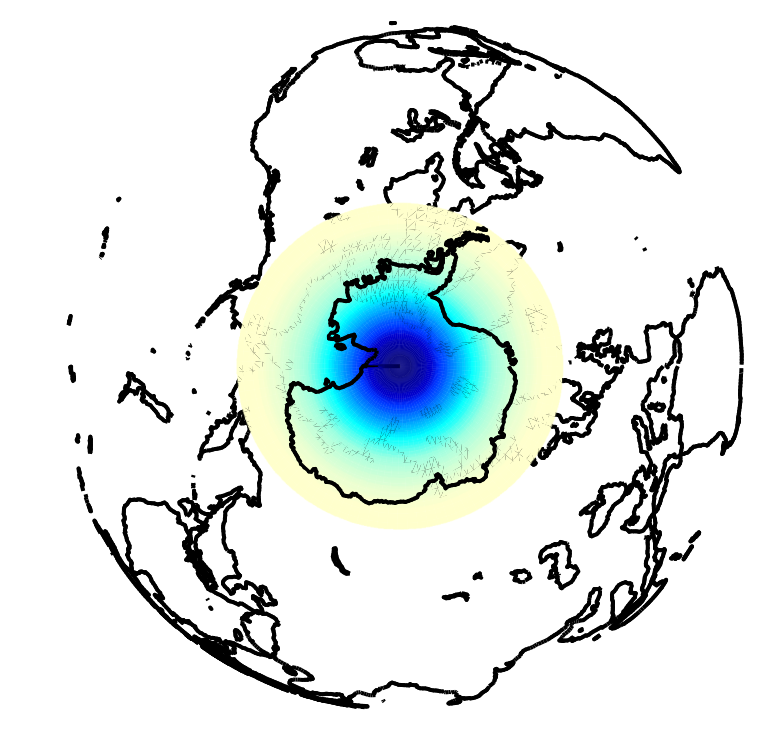
\includegraphics[height=1.2in]{figures/figure3C.png}
  \caption{The first Slepian function of a double polar cap of opening angle 40 degrees plotted in the Mollweide projection (center), on a sphere with the North pole rotated to the center of the image (left), with the South pole rotated to the center (right).}
   \label{figure3}
\end{figure}

\subsection{A Rotated Polar Cap}

If the region of interest is a polar cap or double polar cap that is not axisymmetric and needs to be rotated from the North Pole then a different function is used to produce our matrix of coefficients, \verb|G|.

Run:

\verb|		demos_chapter_two(2.4)|

Instead of \verb|glmalpha()| we are using \verb|glmalphaptoJ()| which requires us to give the following inputs:

\verb|		TH| - the opening angle

\verb|		L| - maximum spherical harmonic degree

\verb|		phi| - the center longitude in degrees of the polar cap of interest

\verb|		theta| - the center colatitude in degrees of the polar cap of interest

\verb|		omega| - the anticlockwise azimuthal rotation in degrees (rotation of the region itself if necessary)

\verb|		J| - the number of Slepian functions to be calculated

This function requires you to know the center colatitude and longitude of your region and to choose the number of Slepian functions to be calculated. For the demo we chose our polar cap to be centered on the antimeridian at the equator, and chose J=50 as we did for earlier examples in which L=20. 

The first Slepian function was evaluated and plotted, however it should be noted that for \textit{glmalphaptoJ()} this does not necessarily correspond to the ``best" concentrated Slepian function overall as in our examples above. Instead, the matrix \verb|G| in this case contains column vectors where the best of every order \textit{m} was calculated first, then the second best of that order, and so forth, repeating this process for each order. So be careful when using this function. 

The plot produced by the demo should match that of figure 4 below:

\begin{figure}[H]
  \centering
  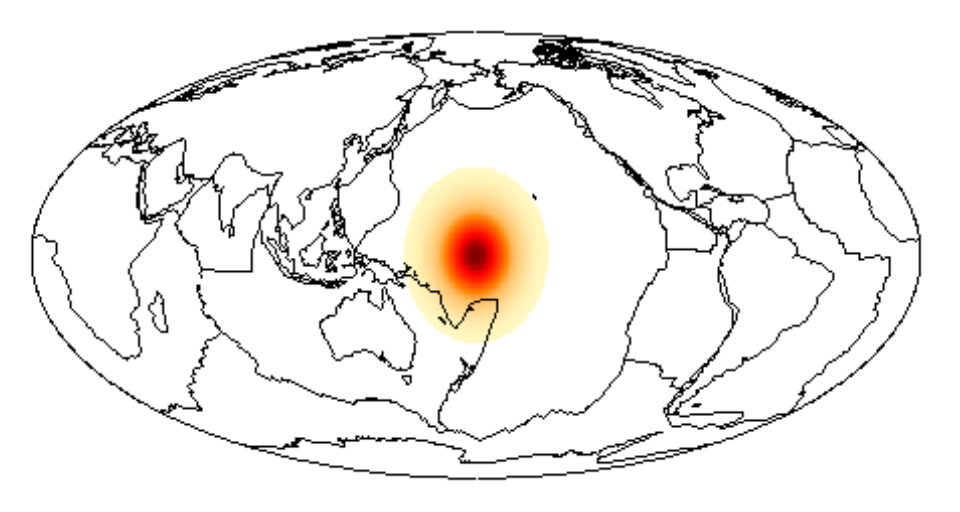
\includegraphics[width=0.5\textwidth]{figures/figure4A.png}
  \caption{The first Slepian function of a polar cap of opening angle 40 degrees plotted in the Mollweide projection. This polar cap has been rotated with its center on the antimeridian at the equator using \textit{glmalphaptoJ()}}
\label{figure4}
\end{figure}


\subsection{Calculating Coefficients for a Polar Ring}

Our next example involves a polar ring, or the difference of two polar caps of different opening angle. 

Run:

\verb|		demos_chapter_two(2.5)|

and observe the output. 

For this demo, \verb|glmalpharing()| was used to produce our matrix of coefficients. \verb|TH| was given to be a vector of two values in degrees \verb|[20 40]| that represent the opening angles of two regions. The difference between these regions is our ring. This function can also accept just one value and calculate a normal polar cap.

\verb|glmalpharing()| only requires three inputs: the opening angle(s) of the polar cap(s), \verb|L|, and a value of 1 to indicate if the \verb|G| matrix will be sorted in order of its eigenvalues (which is also the default input if nothing is specified). 

With plotting you should see: 

\begin{figure}[H]
  \centering
  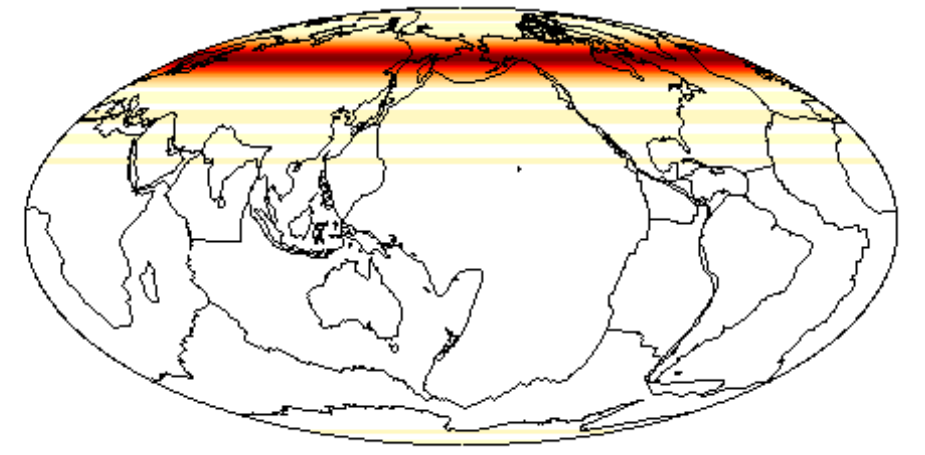
\includegraphics[height=1.2in]{figures/figure5A.png}
  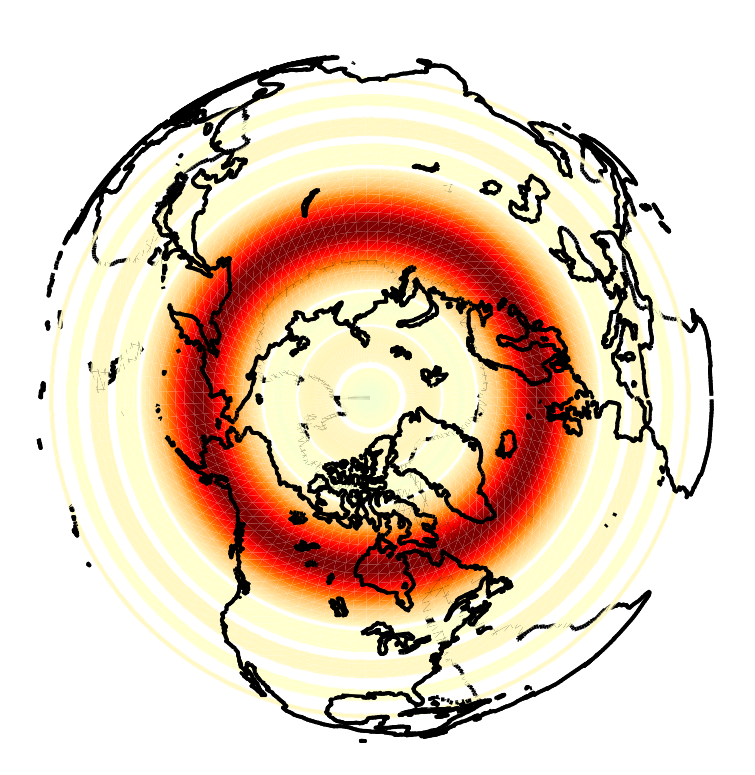
\includegraphics[height=1.2in]{figures/figure5B.png}
  \caption{The first Slepian function of a polar ring which is the difference between two polar caps of opening angle 40 degrees and 20 dgrees, plotted in the Mollweide projection (left) and on a sphere rotated to view the North Pole (right).}
\label{figure5}
\end{figure}



\section{Linear Combinations of Classical Scalar Slepian Functions}

We have been plotting only the first and ``best" concentrated Slepian function within the chosen region for all of the above examples (aside from in example 2.4 with the rotated polar cap). Now we will show how to plot linear combinations of Slepian functions, which can be done for any of the types of regions that we showed above.

Run

\verb|		demos_chapter_two(3.0)|

where we have chosen our region of interest to be North America, expressed by a linear combination of two Slepian functions. To do this, we created a matrix of coefficients using \verb|glmalpha()|. We then combined the first and tenth Slepian functions multiplied by values of 5 and 3 respectively. This sum can be converted into \textit{lmcosi} format in the same line:

\verb|	lmcs=coef2lmcosi((5*G(:,1))+(3*G(:,10)),1);|

The coeficients were then evaluated and plotted in the same methods as above. The demo should produce:

\begin{figure}[H]
  \centering
  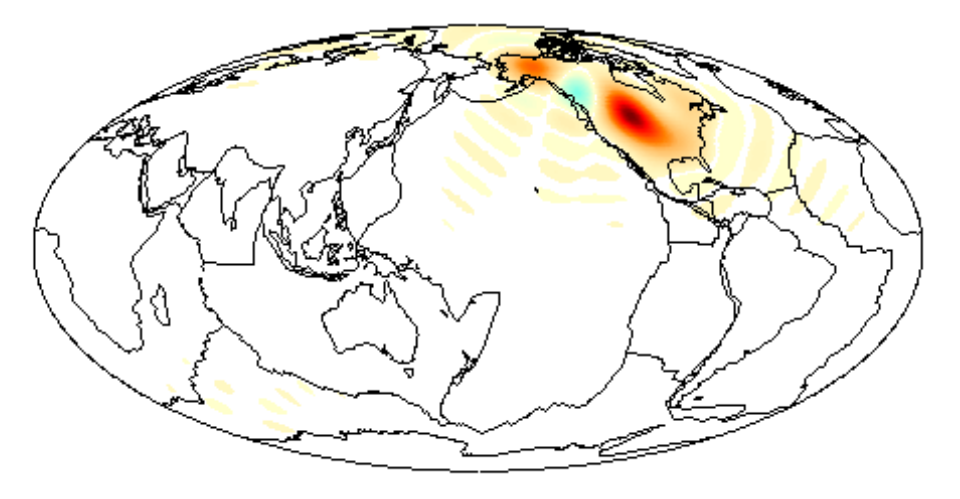
\includegraphics[width=0.5\textwidth]{figures/figure6A.png}
  \caption{A linear combination of Slepian functions plotted for the region North America: $5G_{1} + 3G{10}$.}
\label{figure6}
\end{figure}

Which we can see is starting to look very different from just the first Slepian function.

It should be noted that you can either make linear combinations of coefficients and then evaluate them as we did above, or evaluate the coefficients first, convert to lmcosi format, and then make linear combinations of the Slepian functions.

\textbf{Exercsie:} Practice plotting different linear combinations of slepian functions and observe their output. Try multiplying them by a vector of random coefficients.

\subsection{Using Eigenvalues to Choose the Number of Slepian Functions} 

What if we want more than a combination of a few Slepian functions? How would we choose which functions best represent our region? If you want to know which functions have most of their energy concentrated in the region of interest, we can easily plot their corresponding eigenvalues.

Run

\verb|		demos_chapter_two(3.1)|

which should produce Figure 7, a plot of eigenvalues versus their corresponding Slepian function number.

The eigenvalues are obtained by running \verb|glmalpha()| and ``catching" the second output. We chose North America as our region and kept L=20 as in the previous examples:

\verb|		[G,V] = glmalpha('namerica',20,[],0);|

We then plotted the eigenvalues using:

\verb|		plot(1:((L+1)^2),V);|

and can see in Figure 7 that most of the eigenvalues are approximately 0 past the 50th Slepian function. 

\begin{figure}[H]
  \centering
  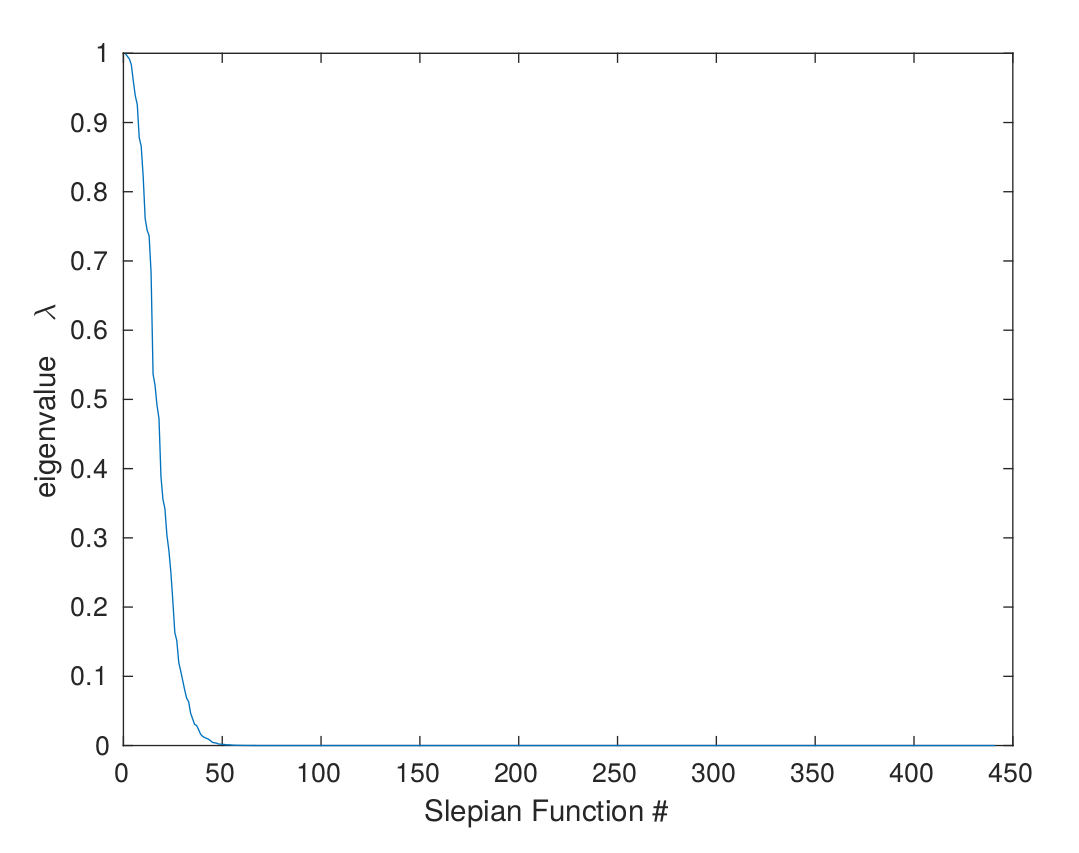
\includegraphics[width=0.5\textwidth]{figures/figure7.png}
  \caption{Eigenvalues plotted on the y-axis versus their corresponding Slepian function number on the x-axis. We can see that most of the energy is occuring in functions corresponding to $j\leq50$.}
\label{figure7}
\end{figure}

In the MATLAB or Octave command prompt you should see that \verb|demos_chapter_two(3.1)| is asking you to choose a value for \verb|J|.  If you choose `50' and hit `enter' the demo will resume and plot the first 50 Slepian functions, producing Figure 8.

In the demo we convert each column of coefficients in \verb|G| to \textit{lmcosi} format, evaluate the coefficients with \verb|plm2xyz|, and place the output as an element in the cell array \verb|g|. This is all done in the following \verb|for| loop:

\verb|for j=1:J| \\
\verb|	g{j} = plm2xyz(coef2lmcosi(G(:,j),1),.5);| \\
\verb|end|

Then we build an empty matrix the same size as \verb|g{1}|:

\verb|	f = zeros(size(g{1}));|

as well as a vector of normally distributed random numbers and length \textit{J} to randomly weight each Slepian function:

\verb|	u = randn(J,1);|

We then use another \verb|for| loop to build our linear combination of the first 50 Slepian functions multiplied by our vector of random coefficients:

\verb|for j=1:J| \\
\verb|	f = f + u(j)*g{j};| \\
\verb|end|

and then feed our matrix \verb|f| into \verb|plotplm()| to make Figure 8. In the figure we see we have a more complex representaion that is still concentrated within North America.

\begin{figure}[H]
  \centering
  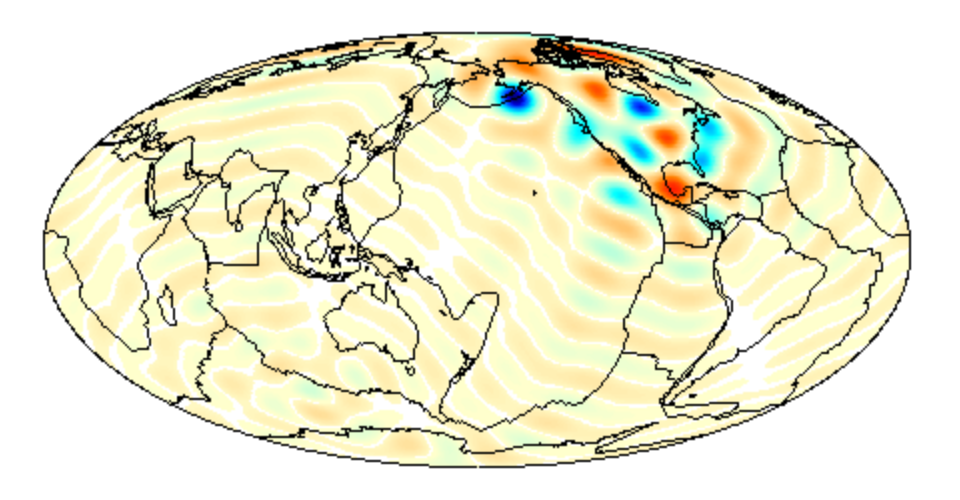
\includegraphics[width=0.5\textwidth]{figures/figure8.png}
  \caption{A linear combination of the first 50 Slepian functions and a vector of normally distributed random numbers plotted for the region of interest North America.}
\label{figure8}
\end{figure}

\textbf{Exercise:} Rerun \verb|demos_chapter_two(3.1)|, choose a different value for \textit{J}, and observe the output. Open \verb|demos_chapter_two.m| in an editor and change the value of \textit{L} in \verb|case 3.1|. Rerun the demo and try different \textit{J} values. 

\TAG
\end{document}
